\documentclass{article}
\usepackage[francais]{babel}
\usepackage[utf8]{inputenc}
\usepackage[T1]{fontenc}
\usepackage{graphicx}
%\usepackage{hyperref}

\begin{document}

\title{Projet TPA Manic Shooter \\ Rapport et documentation}
\author{Boutigny Adrien \& Dechipre Matthieu}
%\date\today
\maketitle

\tableofcontents

\newpage

\section{Introduction}

Le Manic Shooter est un sous genre de Shoot-em-up, une sorte de jeu de tir dynamique est nerveux à base de bullets et de lasers. Cette sous branche à commencé à vraiment sortir du lot dans les années 90 avec des licences célèbres comme Touhou Project en 1996 ou encore DoDonpachi en 1998, des monuments de ce type de jeu.

Celui-ci se différencie des Shoot-em up classiques par certaines caractéristiques. Tout d'abord, la taille du "vaisseau" du joueur se limite dans la plupart des Manic Shooter à un pixel, pourquoi ? Tout simplement pour pouvoir faire face à la deuxième caractèristique phare du Manic Shooter, la multitude de projectiles qui apparaissent à l'écran comme vous pouvez le voir sur cette image tirée de Touhou Project

\begin{center}
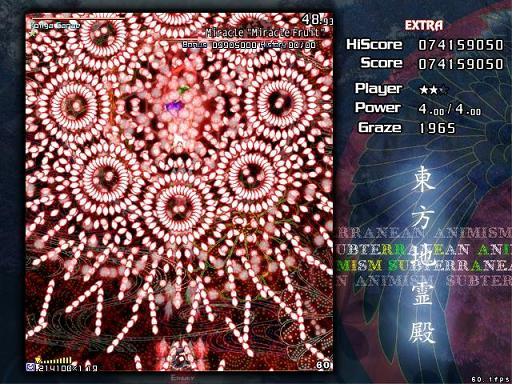
\includegraphics[scale=0.75]{fichiers_rapport/images/touhou_project.jpg}
\end{center}

L'objectif de notre projet est donc le suivant, créer un Manic Shooter. Il faut donc qu'il est les mêmes atouts et défauts que ce dernier. De ce fait, nous avons mis en place un place un moteur de jeu capable de gérer ce nombre immense de projectiles mais aussi d'ennemis.

Dans le cadre de ce jeu, nous avons crée un story-mode, une sorte de mode histoire ou des stages définis à l'avance s'enchainent et où les joueurs pourront tenter d'afficher le highscore. Ce mode se révèle très corsée contrairement au deuxième mode.

Ce deuxième mode en question est un mode où l'on génère de manière procédurale (c'est à dire que l'on imbrique aléatoirement plusieurs vagues d'ennemis prédéfinis) le niveau. Ainsi, en fonction de la difficulté, on obtient un niveau différent à chaque fois.

Suite à plusieurs problèmes, nous avons été obligé de ralentir la progression du jeu et n'avons ajouté des ennemis différents et la gestion du score que très tardivement. La génération de niveau et la majeure partie du moteur de jeu ont été fait pendant le premier semestre et la première moitié du deuxième semestre.

La deuxième moitié du deuxième semestre a été mise à profit pour équilibrer certains ennemis, modifier l'esthétique du jeu, créer de nouveaux ennemis ou encore gérer le highscore et le menu pause.

Nous allons désormais aborder le fonctionnement du jeu et ses mécaniques.

\section{Moteur du jeu}

\subsection{Le générateur de niveaux}

Pour le mode infini de notre jeu, nous avons crée un générateur de niveaux. Ce générateur de niveau se trouve dans le module level.py de notre dépôt et est constitué de plusieurs classes et fonctions. Ce que ce module fait, c'est prendre le contenu des fichiers exemple.dcbbf qui contiennent donc des blocks d'ennemis et va transformer ces blocks en liste d'ennemis qu'il va ensuite mettre bout à bout de manière aléatoire en fonction d'une difficulté (on choisira seulement les blocks dont la difficulté est inférieure ou égale à la difficulté du niveau généré).

Maintenant que nous avons vu de manière assez simple comment nous générons les niveaux, allons plus dans le détail. Tout d'abord, les fichiers .dcbbf.

Un fichier .dcbbf est un fichier qui contient plusieurs informations selon un format bien précis pour permettre au générateur de niveaux de les traiter correctement. Ces fichiers contiennent:

\begin{itemize}
	\item la difficulté de l'ennemi (1)
	\item le niveau de rareté en fonction de la difficulté (2)
	\item les ennemis (3)
\end{itemize}

Comme vous pouvez le voir ci-dessous sur la capture d'écran d'un fichier block:

\begin{center}
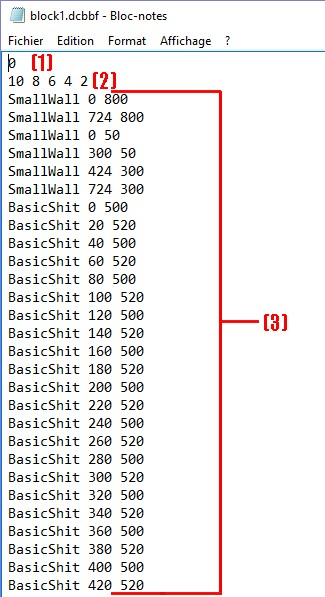
\includegraphics[scale=0.75]{fichiers_rapport/images/explaindcbbf.jpg}
\end{center}

Pour les ennemis normaux, la difficulté va de 0 à 5 et pour les boss de -1 à -5. La difficulté du niveau est aussi l'index qui permettra de définir la rareté du block. En effet, reprenons l'exemple ci-dessus. Si la difficulté choisie pour la création du niveau est de 1, ce block bien précis sera sélectionné car sa difficulté est inférieure à 1. De plus, sa rareté sera fixé à 8 car le générateur va créer une liste de rareté [10, 8, 6, 4, 2] et que l'élément d'indice 1 est 8. Le (3) sera tout simplement la liste des ennemis avec dans l'ordre, le type d'ennemi, la position de sa hitbox en x et la position de sa hitbox en y.

Lorsque l'on voudra créer un niveau, le générateur va charger tous les blocks possibles et ensuite créer deux dictionnaires de fréquence, un pour les blocks standards et un pour ceux des boss. On fait cela car on ne veut qu'un seul boss par niveau à la fin de ce dernier et que de ce fait on ne veut pas qu'il puisse être tiré au hasard parmi les ennemis standards. C'est pour cela que les boss ont des difficulté négatives, on ne s'en sert que pour créer deux dictionnaires différents, sinon, on applique abs(difficulté) - 1 pour pouvoir utiliser correctement leur difficulté.
 
Par la suite, si les blocks ont une difficulté inférieure ou égale à celle du niveau, on les ajoute à leur dictionnaire des fréquences. Pour finir, on va prendre un nombre de blocks aléatoires en fonction de leurs fréquences d'apparition et on va créer une liste d'ennemis à partir des ennemis que le block contient. 

Pour finir, nous parlerons de la gestion des positions des ennemis dans les blocks. Vous avez pu le constater dans l'exemple, tous les ennemis ont leur position en y inférieur à 1000, et les autres fichiers d'ennemis sont pareils. C'est parce que chaque block contient des ennemis sur 1000 pixels, pas plus. Il faut donc prendre ça en compte lorsque nous créons la liste d'ennemis. Pour le premier block, on ne change rien, pour le deuxième block, on ajoute 1000px à tous les ennemis en y, 2000 pour le troisième etc ...

Le schéma ci-dessous résume le processus:

\begin{center}
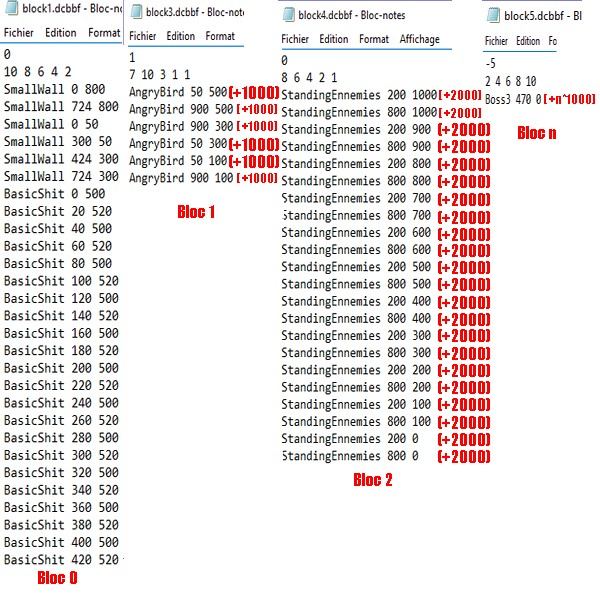
\includegraphics[scale=0.75]{fichiers_rapport/images/explaindcbbf2.jpg}
\end{center}

Comme le générateur fonctionne actuellement, le mode Infini de notre jeu fonctionne par vague de 20 blocks avec un boss à la fin de chaque vague. La difficulté commence à 0 et augmente d'un cran tous les 20 blocks jusqu'à un maximum de 4.

\section{Deuxième partie}



\section{Réalisation}

\subsection{Environnement}

Notre jeu est codé sous Python 3

\section{Conclusion}

\section{Suppléments}

\subsection{Sources}

\noindent https://www.libsdl.org/ \newline
https://www.python.org/download/releases/3.4.0/ \newline
https://bitbucket.org/pyglet/pyglet/wiki/Home

\subsection{Documentation}

\noindent http://www.developpez.com/ \newline
https://openclassrooms.com/ \newline
https://pysdl2.readthedocs.org/en/latest/ \newline
https://pyglet.readthedocs.org/en/pyglet-1.2-maintenance/

\end{document}
